\section{Schätzen}

\subsection{Eigenschaften von Schätzern}

\subsubsection{Konsistenz}

Korrektur für genügend grosse Stichproben
$$ \lim\limits_{n \to \infty} \hat{\vartheta}(x_1, \, \ldots \, , \, x_n) = \vartheta $$


\subsubsection{Erwartungstreu}

Im Mittel korrekt selbst für kleine Stichproben
$$ E (\hat{\vartheta}(X_1, \, ... \, , \, X_n) ) = \vartheta $$


\subsection{Maximum Likelihood Prinzip}

\subsubsection{Aufgabe}

Stichprobe $x1, \, \ldots \, , x_n$ einer normalverteilten Zufallsvariable mit $\sigma = 1$. \\
Schätze den Parameter $\mu$ der Standardnormalverteilung
$$ \cbl{\varphi}(x, \crd{\mu}) = \frac{1}{ \sqrt{2 \pi}} e^{- \frac{(x - \crd{\mu})^2}{2}}  \, \diff x $$


\subsubsection{Likelihood-Funktion}

\begin{minipage}{0.4\columnwidth}
    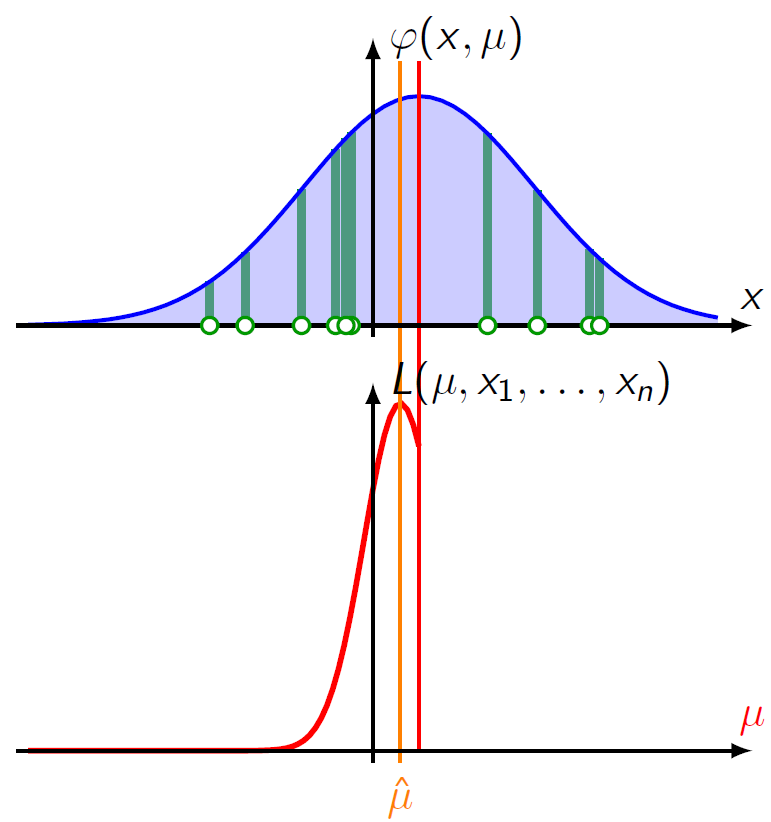
\includegraphics[width=\columnwidth]{images/likelihood.png} 
\end{minipage}
\hfill
\begin{minipage}{0.5\columnwidth}
    Bewerte Kandidaten $\crd{\mu}$ mit der Likelihood-Funktion 

    $$ L(\mu, x_1, ... x_n) = \cgn{\varphi(x_1, \mu)} \, ... \,  \cgn{\varphi(x_n, \mu)} $$
    $$ \text{ \textrightarrow\ } \cor{\hat{\mu}} = \mathrm{arg \, max}_{\substack{\mu}} L(\mu, x_1, ... x_n) $$
\end{minipage}

\vspace{0.2cm}

\myul{\textbf{Likelihood-Funktion}}
$$ L(\vartheta, x_1, ... x_n) = \varphi(\vartheta, x_1) \cdot \varphi(\vartheta, x_2) ... \varphi(\vartheta, x_n) $$
Wahrscheinlichkeit für die Werte $x_i$ 

\vspace{0.2cm}

\myul{\textbf{Prinzip}}
\vspace{0.1cm}

$\hat{\vartheta}(x_1, ..., x_n)$ maximiert  $L(\vartheta, x_1, ... x_n)$ (Maximum-Likelihood-Schätzer) \\
\textrightarrow\ Ableiten und Null setzen!


\example{Schätzung von $\bm{\mu}$}

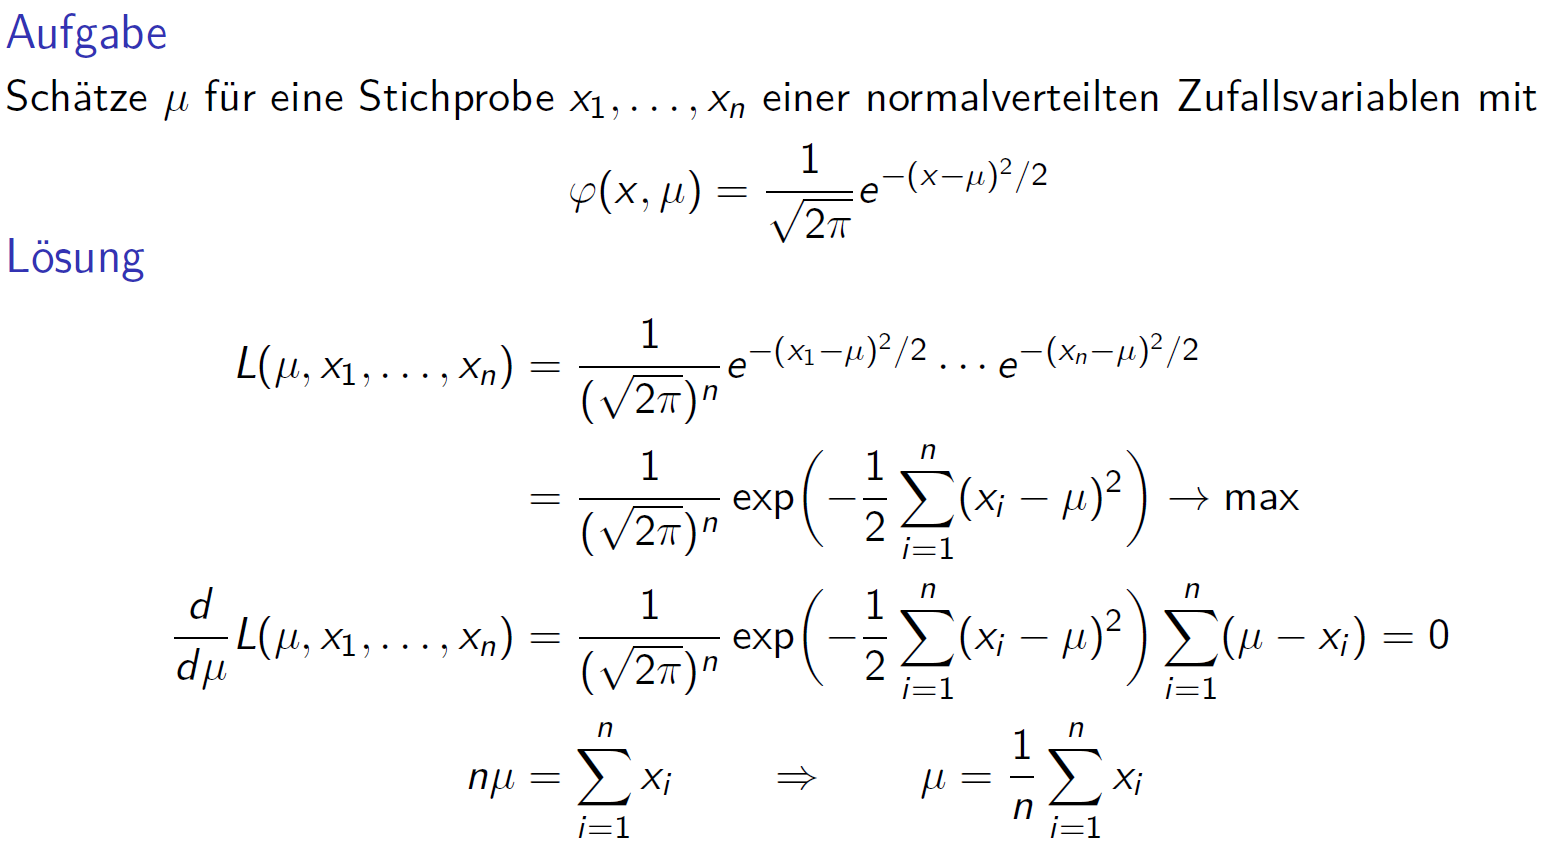
\includegraphics[width=\columnwidth]{images/likelihood_beispiel.png}


\subsection{Konfidenzintervall}

 $[\vartheta_-, \vartheta_+]$ heisst \textbf{Konfidenzintervall} zum (Vertrauens-)Niveau $1 - \alpha$ 

\vspace{0.2cm}

\myul{\textbf{Aufgabe:}}

\vspace{0.1cm}

Finde ein Intervall $[\vartheta_-, \vartheta_+]$, das den wahren Wert des Parameters mit Wahrscheinlichkeit $1 - \alpha$ enthält.

\vspace{0.2cm}

\begin{minipage}{0.4\columnwidth}
    \includegraphics[width=\columnwidth]{images/Konfidenzintervall}
\end{minipage}
\hfill
\begin{minipage}{0.55\columnwidth}
    \myul{\textbf{Lösung}}

    \vspace{0.1cm}

    \begin{itemize}
        \item  Verteilung von $\vartheta$: \\
            Wahrscheinlichtsichte $\varphi(\vartheta)$ und Verteilungsfunktion $F_{\vartheta}$
        \item Finde $\vartheta$-Werte so, dass $1 - \alpha = F(\vartheta_+) - F(\vartheta_-)$
    \end{itemize}
\end{minipage}


\subsection{Intervallschätzung}

\myul{\textbf{Aufgabe}}

\vspace{0.1cm}

Gegeben eine normalverteilte Stichprobe $X_i$, $i = 1, \, \ldots \, n$ 
Finde ein Intervall, welches $\mu$ mit Warhscheinlichkeit 95\% enthält.
$$ \hat{\mu} = \frac{1}{n} (X_1 + \ldots + X_n) $$


\subsubsection{Lösung 1 - Bekannte Varianz}

$\hat{\mu}$ ist normalverteilt mit Erwartungswert $\mu$ und Varianz $\frac{1}{n} \sigma^2$

$$ \boxed{ \left[ \hat{\mu} - 1.96 \frac{\sigma}{\sqrt{n}} \, , \, \hat{\mu} + 1.96 \frac{\sigma}{\sqrt{n}}  \right] } $$

Das angegebene Intervall enthält $\mu$ mit Wahrscheinlichkeit 95\%


\subsubsection{Lösung 2 - Geschätzte Varianz}

$$ \boxed{ t = \frac{\hat{\mu} - \mu}{\hat{\sigma} / \sqrt{n}} \quad \text{t-verteilt mit } k = n-1 \text{ Freiheitsgraden} } $$

Finde ein Intervall $[t_- \, , \, t_+]$, das $t$ mit Wahrscheinlichkeit 95\% ethält. \\ 
Dann ist das gesuchte Intervall:

$$ \boxed{ \left[ \hat{\mu} + t_- \frac{\hat{\sigma}}{\sqrt{n}} \, , \, \hat{\mu} + t_+ \frac{\hat{\sigma}}{\sqrt{n}}  \right] } $$

\textbf{ \textrightarrow\ $\bm{t}$-Tabelle siehe Abschnitt \ref{Quantilen der t-Verteilung}}
